\section{Central Computer}\label{sec:CC:design}
Dette afsnit omhandler designet af "Central Computer" som i sin naturlig er design af den software som skal køre på den den embedded controller beskrevet i afsnit  \ref{sec:Embedded_Controller}. Da UC1 og UC2 kun adskiller sig ved at SumoBots er styret af hhv. mikrofon og joystik, at her valgt at dokumentere designet af central computer igennem UC1. På det tekniske plan vil designet til UC2 være identisk for central computer da denne modtager signalet om retning og hastighed fra styringsenheden efter samme protokol og ændringer fra UC1 til UC2 derfor udelukkende foregår på styringsenheden.  


\section{Use Case 1}
På baggrund af domæneanalysen som ses på figur \ref{fig:RSB_Domænemodel} er der udarbejdet først en applikationsmodel\cite{ApplikationsmodellerI2ISE} som indledningsvist bestod af et konceptuelt klassediagram, direkte på baggrund af interfaces beskrevet på i IBD'et på figur \figref{Strukturering/Robo-Sumo-Battle/IBD_Robo_sumo_battle.pdf} såvel som domænemodellen udarbejdet på baggrund af UC1. Det konceptuelle klassediagram indeholder de samme klasser som det endelige klassediagram, blot uden funktioner - de er fastlagt igennem de sekvensdiagrammet for use casen.

\subsection{Sekvensdiagram}
For use casen er der udarbejdet et sekvensdiagram hvorigennem funktionsnavne og -parmetre er fastlagt, som ses på figur \ref{fig:CC_SD_UC1}. Sekvensdiagrammer er udarbejdet stringent på baggrund af sekvensen i use casen. Fordi sekvensdiagrammer er udarbejdet stringent ift. use casen er der trivialiteter og programmeringstekniske overvejelser som er udeladt til fordel for oveblikket i diagrammet. Implementeringen tager således afsæt i diagrammet og der vil være en stærk sekvensmæssigt vil relation mellem sekvensdiagrammet og koden - om end der vil formentligt vil kunne findes ændringer. Sekvensdiagrammet vil blive implementeret i funktionen UC1::Run(). 

\begin{figure}
    \centering
    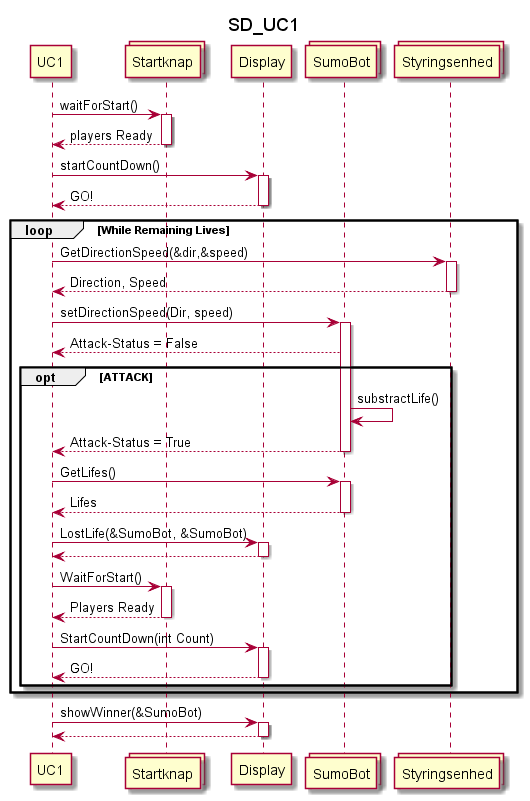
\includegraphics[width=\textwidth]{figs/Design/Central Computer/SekvensDiagrammer/SD_UC1.png}
    \caption{Sekvensdiagram for Central Computer i UC1}
    \label{fig:CC_SD_UC1}
\end{figure}

\subsection{Klassediagram}
På baggrund af sekvens-diagrammets funktioner og funktionskald på tværs af klasser er der udformet et klassediagram med relevante funktioner og relationer, som ses i figur \ref{fig:CC_CD_UC1}. 

\begin{figure}
    \centering
    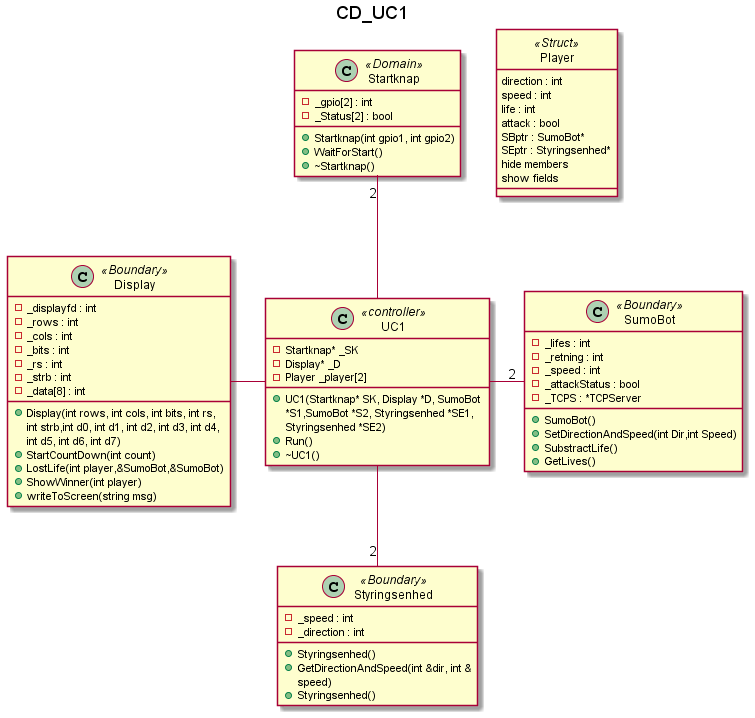
\includegraphics[width=\textwidth]{figs/Design/Central Computer/applikationsmodel/CD_UC1.png}
    \caption{Klassediagram for Central Computer i UC1}
    \label{fig:CC_CD_UC1}
\end{figure}

\subsubsection{Player}
\label{subsubsec:Player}
På klassediagrammet ses også en struktur (struct) kaldet Player, som indeholder vigtig information om hver spiller. Strukturen Player er dannet med henblik på at give mulighed for en implementering hvor loopet afbilledet i sekvensdiagrammet figur \ref{fig:CC_SD_UC1}, "While Remaining Lives" kan blive en løkke som gentager sig for hver spiller, hvis information og pointersså kan ligger gemt i et array - hvert gennemløb af loopet kan så skiftevis være for player ét og 2.Således bliver koden halvt så lang, mere overskuelig og det vil med samme kode blive let at tilføje flere spillere.  

%%%%%%%%%%%%%% Klassen UC1 %%%%%%%%%%%%%%%%%%%

\subsubsection{UC1}
UC1 er controllerklassen \cite{ApplikationsmodellerI2ISE} igennem hvilken use case 1 eksekveres. 
\paragraph{Attributter}
UC1 skal for at kunne benyttes bruge pointers til klasserne Startknap og Display. Derudover skal der for hver spiller også bruges en henvisning til en klasse af typen SumoBot og Styringsenhed - dette gemmes bla. i strukturen Player, som UC1 klassen benytter 2 af. 
\paragraph{Metoder}
I dette afsnit vil klassen UC1's metoder blive beskrevet. 

\begin{functionDescription}
{UC1::UC1(Startknap* SK, Display* D, SumoBot* SB1, SumoBot* SB2, Styringsenhed* SE1, Styringsenhed* SE2)}
{func:UC1_constructor}
{UC1 constructoren sætter den række pointers som nævnt i attributter såvel som liv til at starte på 3. Skriver iøvrigt "Welcome to Robo Sumo Battle" ud på displayet}
{\begin{itemize}
    \item \textbf{Startknapt* SK:} Reference til et Startknap objekt. 
    \item \textbf{Display* D:} Reference til et Display objekt
    \item \textbf{SumoBot* SB1:} Reference til det SumoBot objekt som repræsenterer den SumoBot som skal styres af Player 1
    \item \textbf{SumoBot* SB2:} Reference til det SumoBot objekt som repræsenterer den SumoBot som skal styres af Player 2
    \item \textbf{Styringsenhed* SE1:} Reference til den det Styringsenhed objekt som repræsenterer den styringsenhed som skal Player 1 benytter
    \item \textbf{Styringsenhed* SE2:} Reference til den det Styringsenhed objekt som repræsenterer den styringsenhed som skal Player 2 benytter
\end{itemize}}
{Returnerer et UC1 objekt}
\end{functionDescription}

\begin{functionDescription}
{UC1::Run}
{func:UC1_run}
{Dette er funktionen som eksekverer UC1 med de angivne enheder i constructoren. Funktionens sekvens holder sig stringent til sekvensdiagrammet som ses i figur \ref{fig:CC_SD_UC1}}
{N/A}
{N/A}
\end{functionDescription}

\begin{functionDescription}
{UC1::~UC1()}
{func:destructor_UC1}
{Destructor for UC1 som blot skriver "Goodbye..." ud på skærmen}
{N/A}
{N/A}
\end{functionDescription}

%%%%%%%%%%% Klassen Startknap %%%%%%%%%%%%%%5

\subsection{Startknap}
Klassen Startknap har til formål at interface og interagere med de to startknapper, som fysisk sidder ifm. de to styringsenheder, hvorpå de to spillere kan angive at de er klar til at spille. 

\textbf{Prerequisites:}
Startknap gør brug af biblioteket wiringPi\cite{2020Http://wiringpi.com/}.

\paragraph{Attributter}
Klassen Startknap indeholder en attribut til hhv. at indeholde status for hvorvidt de to respektive spillere har tilkendegivet at de er klar til at starte spillet, på hver deres startknap og en attribut til at indeholde information om hvilken GPIO-port på den embedded controller som startknappen er tilsluttet. 

\begin{functionDescription}
{Startknap::Startknap(int gpio1, int gpio2)}
{func:Startknap_constructor}
{Startknappens constructor initialiserer funktionerne i wiringPi\cite{2020Http://wiringpi.com/}, sætter attributten \textit{gpio} og sætter disse som udgang.
}
{\begin{itemize}
    \item \textbf{int gpio1:} GPIO'en på den embedded controller hvorpå den ene startknap er tilslutte. Bemærk at GPIO nummereringer er foretaget på baggrund af wiringPi bibliotekets nummerering\footnote{http://wiringpi.com/pins/}. 
\end{itemize}}
{N/A}
\end{functionDescription}

\begin{functionDescription}
{void Startknap::waitForStart()}
{func:Startknap_waitForStart}
{Funktionen foretager "busy waiting" indtil begge spillere har tilkendegivet at de er klar til at spille på deres startknap og tager iøvrigt udgangspunkt i at startknapperne er aktivt høje. Funktionen husker tilkendegivningerne således at de to spillere ikke behøver at tilkendegive at de er klar samtidig}
{N/A}
{N/A}
\end{functionDescription}

\begin{functionDescription}
{Startknap::~Startknap()}
{func:Startknap_destructor}
{Klassen Startknap benytter en default destructor da wiringPi's API ikke stiller krav til at skulle frigive GPIO'erne}
{N/A}
{N/A}
\end{functionDescription}

%%%%%%%%%%%%% Klassen Display %%%%%%%%%%%%%%%%%5
\subsection{Display}
Klassen display håndterer kommunikationen på displayet. Klassen er lavet med metoder med prædefinee tekster således at der fra use case klasserne blot skal kaldes eksempelvis én funktion med et heltal, for at vise en nedtælling. En funktion gør brug af hjælpeklassen lcd.h fra biblioteket wiringPi\cite{2020Http://wiringpi.com/}, men har sin egen logik til at flytte cursoren på LCD skærmen såvel og parse strings ud på denne. 

\textbf{Prerequisites:} wiringPi biblioteket fra hvilket der er benyttet metoder til at initialisere GPIOs, flytte LCD-cursoren og overføre enkelte bogstaver.

\paragraph{Attributter}
\begin{itemize}
	\item \textbf{int \_displayfd:} En filedescriptor som fungerer som \textit{handle} til displayet. 
	\item \textbf{int \_rows:} Antallet af rækker som det tilsluttede display har
	\item \textbf{int \_cols:} Antallet af kolonner som det tilsluttede display har
	\item \textbf{int \_bits:} Antallet af bits som bruges til at interface displayet (4 eller 8)
	\item \textbf{int \_rs:} Repræsenterer den GPIO på embedded controller som er forbundet til displayets RS-pin\footnote{Register Select}
	\item \textbf{int \_strb:} Repræsenterer den GPIO på embedded controller som er forbundet til displayets Strobe-pin\footnote{Pin til at opdatere displayet}. 
	\item \textbf{int \_data[8]:} Repræsenterer de 8 GPIO'er på embedded controller som er forbundet til displayets data-pins.
\end{itemize}
\paragraph{Funktion()}

\paragraph{\~Funktion()}
\begin{functionDescription}
{Display::Display(int rows, int cols, int bits, int rs, int strb, int d0, int d1, int d2, int d3, int d4, int d5, int d6, int d7)}
{func:Display_constructor}
{Display klassens constructor initialiserer først og fremmest klassen attributter på baggrund af parametrene. Parmetrene benyttes her også til at initialisere LCD-pins vha. metoder fra wiringPi-biblioteket}
{\textit{Se attributter}}
{N/A}
\end{functionDescription}

\begin{functionDescription}
{int Display::writeToScreen(string msg)}
{func:Display_writeToScreen}
{Denne funktion kaldes som udgangspunkt kun af andre funktioner i klassen og kan ansees som en utiliti-funktion, som klassens resterende metoder kan benytte sig af. Funktionen tager den modtagne streng og indledningsvist validerer hvorvidt den kan være på skærmen. Herefter skiftevis skrives et bogstav ud på skærmen og cursoren flyttes tilsvarende hen over skærmens kolonner og rækker. Hvis cursoren møder et newline-character, gås til næste række og der tjekkes løbende om cursoren prøver at overskride den sidste kolonne i sidste række.}
{\textbf{string msg:} Den streng som ønskes skrevet ud på displayet}
{Der returneres -1 for en tekst der er for lang, -2 for en forsøg på at overskride sidste række's sidste kolonne og 0 for succesfuld udskrift på skærmen}
\end{functionDescription}

\begin{functionDescription}
{void Display::startCountDown(int count)}
{func:Display_startCountDown}
{Funktionen viser en nedtælling på skærmen fra det tal som medsendes som parameter. Funktionen benytter busywait fra Linux' egne biblioteker}
{\textbf{int count:} Tallet i sekunder som der skal tælles ned fra}
{N/A}
\end{functionDescription}

\begin{functionDescription}
{void Display::lostLife(int player, SumoBot *S1, SumoBot *S2)}
{func:Display_lost_life}
{Funktionen udskriver på skærmen at en SumoBot har tabt et liv, hvilken SumoBot der har mistet et liv samt den nuværende stilling. Det bemærkes at metoden bygger på at der kun er to spillere - det vil være muligt at modificere denne til at modtaget et UC-objekt som vha. en get-metode vil kunne formidle adgang til \_player-arrayet hvorfra der vil kunne hentes information om flere SumoBot's liv. I denne iteration vil der for simpliciteten blot kunne vises for 2 spillere. 
}
{\begin{itemize}
    \item \textbf{int player:} Hvilken spiller der har mistet et liv. 
    \item \textbf{SumoBot* S1:} Pointer til det ene SumoBot objekt.
    \item \textbf{SumoBot* S2:} Pointer til det andet SumoBot objekt. 
\end{itemize}}
{N/A}
\end{functionDescription}

% \begin{figure}
%     \centering
%     \includegraphics[width=\textwidth]{}
%     \caption{}
%     \label{fig:}
% \end{figure}

% \subsection{Klasse}
% \paragraph{Attributter}
% \paragraph{Funktion()}
% \paragraph{\~Funktion()}

% \begin{functionDescription}
% {Navn}
% {func:label}
% {Beskrivelse}
% {Parametre}
% {Returværdi}
% \end{functionDescription}